
\chapter{Orientation anisotropies in the inputs to the primary visual cortex of macaques}

\pagebreak

	\section{Abstract}
	
			The neurons of the primary visual cortex are arranged in columns based on their orientation preference. The columnar architecture has orientation columns that cycles through all the orientations and converge at a pinwheel centre. It has recently been proposed that both this columnar organisation and the orientation selectivity of individual neurons can be established from broadly tuned subcortical inputs. While this has to some extent been demonstrated in intracellular recordings, the overall nature of these inputs is yet to be studied. In this study, I will be using optical imaging of intrinsic signals to characterise these inputs. The columnar architecture first revealed using extracellular recordings but was further confirmed using optical imaging of intrinsic signals (OI). OI detects the haemodynamic change that accompanies neural activity. A lower level of oxygenated blood would indicate higher activity. Traditionally the signal from the OI is spatially filtered in order to isolate activity in the relevant spatial scale; activity that corresponds to the output of the neurons. Here I use the unfiltered signal to reveal activity that is more congruent with the pre-synaptic and synaptic activity. When examined this way in the anaesthetised macaque primary visual cortex, the unfiltered signal is tuned to the radial orientation (the orientation the receptive field makes with the visual field). These results show that inputs to the cortex are biased toward the radial orientation, a bias that has been observed in both the retina and LGN of the macaque.
\pagebreak

	\section{Introduction}
	
	Neurons in the primary visual cortex are tuned to orientation and these orientation tuned neurons are organised in columns. Hubel and Wiesel (1962) showed that neurons in Area 17 of cats were sharply tuned to orientation. These neurons were also grouped into neurons of similar orientation. This was then repeated in macaques. Hubel and Wiesel suggested their excitatory convergence model for orientation tuning. This model suggests that orientation tuning in the primary visual cortex is established by the feedforward convergence of inputs from neurons arranged in a row in the lateral geniculate nucleus (LGN). Now, the orientation selectivity and the columnar architecture is a widely accepted characteristic of the primary visual cortex of most species (see mouse work for an alternative scheme, (Reference)). However, the question remains as to whether both these properties arise from the same mechanism.


	A study by Sur et al. (2001) showed that simple feedforward mechanisms were not effective in establishing the columnar architecture observed in the primary visual cortex. Where they routed signals from the V1 to the auditory cortex, they found that orientation tuning was sharpened (although not enough) by the feedforward mechanism but the cortical architecture of V1 was not reflected in the auditory cortex, implying that intracortical intervention was necessary for establishing cortical architecture as we know it. A new theory (Vidyasagar and Eysel, 2015) suggested that both the orientation tuning of cortical neurons and cortical architecture can be established by sharpening biases that originate earlier on in the visual system.
	
	
	Let us examine the way the visual system processes colour data. Colour is encoded in the retina by cones with broad sensitivities that act in an opponent manner to each other. So, there is the red/ green opponent system and blue/ yellow opponent system encoded by the L, M and S cones. These cones are activated by a light of a large range of wavelengths. Neurons in the primary visual cortex (V1) that are tuned to colour however, only respond to particular wavelengths of light. This tuning in the primary visual cortex arises from a sharpening of the broader bias established in the retina. A similar mechanism has been reported for other features that have been observed in the V1. Neuronal properties such as ocular dominance and phase selectivity (on/off) can all be explained by biases established by biases observed in the retina. A similar mechanism may be proposed for orientation selectivity.
	
	
	The case of orientation selectivity is more complex than ocular dominance or phase selectivity. The nature of ocular dominancy and phase selectivity is such that the seed for their tuning in the retina is quite intuitive and commonly accepted. Inputs may either be from the right eye or the left eye. They may arise from a ganglion cell that receives inputs from an on or off bipolar cells. These biases are well characterised in the literature. In the case of orientation selectivity however, the sub-cortical biases are not so obvious. While many studies have shown that sub-cortical neurons are indeed biased for orientation (eg: see Levick and Thibos, 1980; Vidyasagar and Urbas, 1982) it is still not widely accepted. Several studies continue to argue that orientation selectivity is first generated in the primary visual cortex through some variant of the excitatory convergence model. Further, the exact nature of the bias is still questioned. Some studies suggest that there is radial orientation bias in the retina. Some others suggest that there is a preponderance of the horizontal and vertical orientation biases (the oblique effect). Rovamo et al (1978) showed an eccentricity dependence of perceptual bias with the central vision showing oblique effect and peripheral vision showing the radial bias. One study in the cat area 17 showed that first order neurons in layer 4 of the cortex were tuned to cardinal orientations. Cardinal orientations were defined as vertical, horizontal or radial. It could be that the retinal neurons are tuned for one of these cardinal orientations which are reflected in the first order neurons in the cat visual cortex.
	
	
	One of the key tools that have been instrumental in revealing cortical architecture is optical imaging of intrinsic signals (OI). Introduced in the 90s, OI helped visualise the cortical orientation columns converging at a pinwheel centre. OI images the haemodynamic change that accompanies neural activity and is based on the principle that deoxygenated blood reflects less light than oxygenated blood. This means that activity is observed as dark areas in the response maps. The haemodynamic change that is recorded using OI is akin to the BOLD (Blood Oxygen Level Dependent) response observed in fMRI. Studies have suggested that the BOLD response is predominantly a reflection of the pre-synaptic and synaptic activity with the extracellular, spiking activity forming a very small part of the response. The OI images that we observe are reflections of the spiking activity. This is because, traditionally OI signal is spatially filtered to only display the spiking activity. Here, I aim to use the non-filtered signal to study the pre-synaptic and synaptic activity in the macaque V1. Using optical imaging helps reveal any larger scale organisation that cannot be otherwise observed. 
	
	Hypothesis:


	- If cortical orientation tuning and architecture were derived from broadly orientation inputs, then the unfiltered OI response will be tuned to one of the cardinal orientations.


	- If however, the orientation biases in the inputs were derived from a mechanism such as excitatory convergence, the unfiltered OI response will show no such preponderance.
	
	
	\pagebreak
		
	\section{Methods}
	
	\subsection{Data Collection}
		
		\subsubsection{Stimulus}	
		
		During the experiment OI maps were calculated in response to visual stimulation. Visual stimulus was generated using the Visual stimulus generator (SDL, Cambridge Research Systems, UK) and presented on a Barco monitor (Reference Calibrator plus; Barco Video and Communications, Belgium).  The monitor was positioned at 57 cm from the animal. The stimulus presented was a full field, square-wave, bidirectional, drifting grating (SF= 1-4 cpd, TF= 1.5 Hz, Michelson contrast= 100\%). The orientation of the grating changed sequentially in 22.5 degree steps from 0 degrees to 157.5 degrees. A 0 degree grating was a horizontal grating moving bidirectionally. The stimulus was presented for 7.3 seconds followed by an interstimulus interval of 10 seconds where the animal viewed a blank screen.
		
		\subsubsection{Optical Imaging of intrinsic signals}
				
			Optical imaging of intrinsic signals was used to obtain the haemodynamic change related to the neural response to orientation stimuli. The OI setup involved two camera lenses (Canon) arranged in a tandem fashion (Reference) connected to a CCD camera. The tandem lens arrangement allowed for a narrow plane of focus. An LED light source was used to illuminate the cortical surface. Before stimulus presentation, a high contrast, ‘green image’ of the surface of the imaged cortex was obtained by illuminating the cortical surface with green light (filter wavelength=545 nm). This provided us with cortical landmarks which were later used in determining the locations for electrode tracks for topographical recordings. Following this, the plane of focus of the camera setup was changed to between 550-700 microns beneath the surface of the cortex and the wavelength of the illuminating light was changed to 630 nm. 18 frames, each 400 ms long were collected for each stimulus presentation. The signal to noise ratio was enhanced by acquiring data over 50 trials collected in 10 blocks of 5 trials each. Where possible, given the condition of the imaged area and the animal, the experiment was repeated a second time. Using the OI data acquisition system, each block was exported as a MATLAB file. Each individual frame in a block was the average of that frame for 5 trials. Analysis was conducted on the exported MATLAB files.
		
			
		\subsubsection{Topographical recordings}
	
			The study of radial bias requires the careful plotting of receptive field locations in relation to their cortical location. High impedence tungsten microelectrodes (12 MOhm, FHC Inc) were used to record from predetermined locations on the imaged cortical surface). The analog signal was amplified and filtered (Amplifier specs; Gain = x10,000; Band pass between 300 and 3000 Hz). The filtered signal was then visualised using an oscilloscope (Oscilloscope specs) and fed through an audio speaker to aid in plotting the receptive fields. First the foveal location (if visible) and the optic nerve with blood vessel markers were plotted using a fundus camera (Fundus Camera specs). Then the location of the receptive fields were carefully hand plotted using handheld stimuli from the corners of the imaged area (See figure 3). In between each electrode penetration, where possible, the location of the fovea and optic nerve head were replotted in order to account for eye movement.
			
			
	\subsection{Data Analysis}
		\subsubsection{Image Analysis}

			Of the 18 frames collected, the mean of 14 frames ( frames 3-16) was calculated for individual blocks in each stimulus condition. The first frame was then subtracted from the averaged frames for each stimulus condition. The mean of 10 blocks was then calculated. This gave us the unfiltered single condition maps (referred to as veridical SCMs). Traditionally, when analysing the images obtained using optical imaging of intrinsic signals, the following method is used. The veridical SCMs are band pass filtered using the method described in figure 6.1. The unfiltered map is first low pass filtered using a large spatial filter (Gaussian filter, sigma= 312.5 microns). This removes the low frequency information. By subtracting the low pass image calculated above from the original image, we preserve only the high spatial frequency information. This will be called the high-pass single condition map. The high pass single condition map is then smoothed with a gaussian filter with a smaller sigma value (100 microns). This is the band pass filtered single condition map or more commonly just referred to as the single condition map (these will be referred to as filtered SCMs throughout this thesis). The filtered SCMs are then vector averaged to look at the angular mean of individual pixels (Swindale). This will produce the traditional filtered orientation tuning maps. In our study, we also vector averaged the veridical SCMs. We called the maps derived this way the veridical orientation maps (see appendix for code).
			
			\begin{figure}
			
				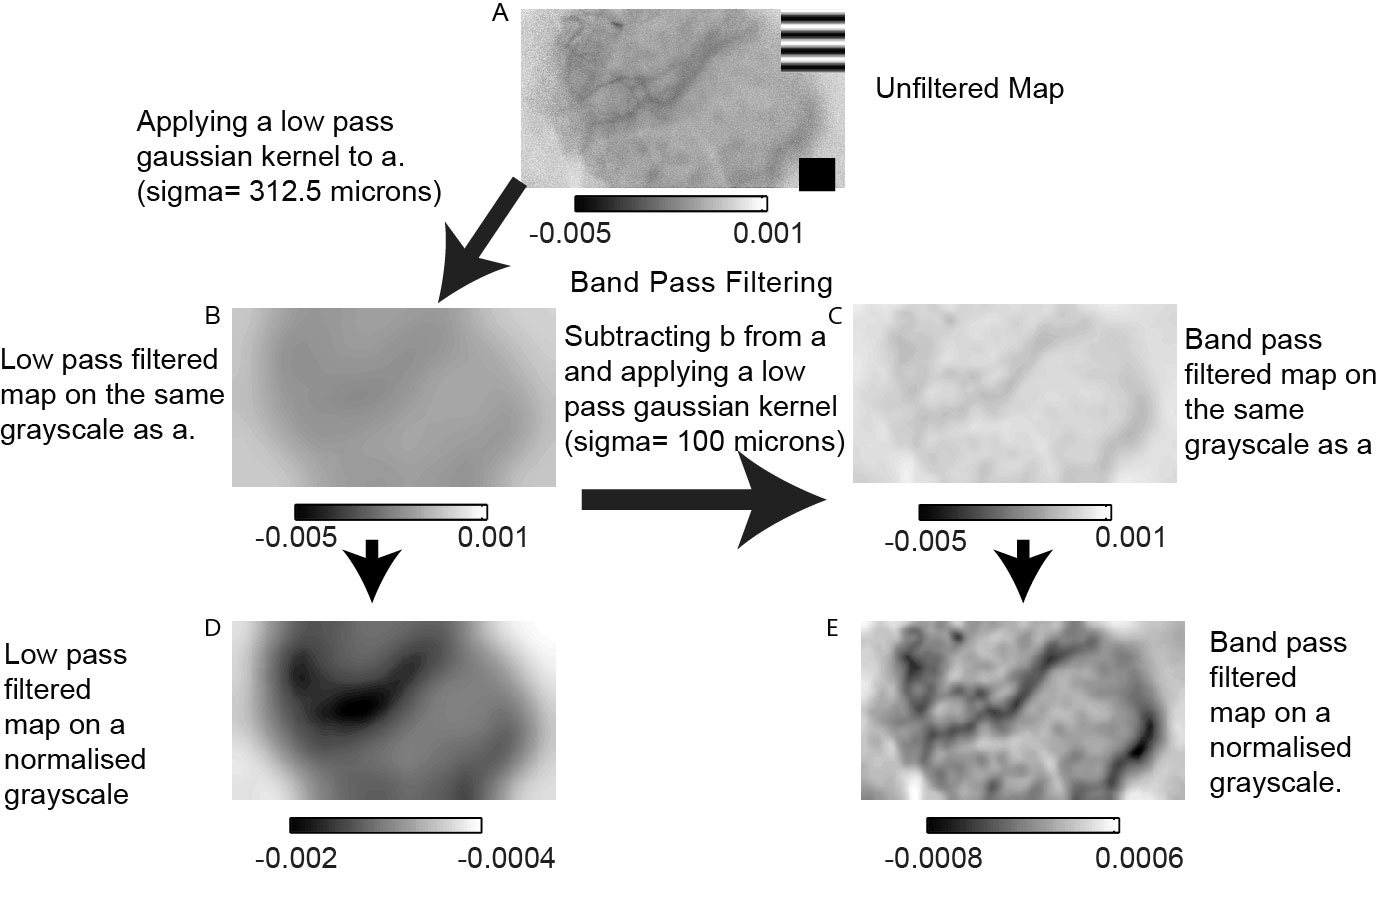
\includegraphics[width=\linewidth]{rb/filtering.jpg}
				\caption{Figure 1: Description of the filtering process. A low pass Gaussian filter ($\sigma$=312.5 $\mu$m) is applied to the unfiltered single condition map (SCM; (a)) to obtain the low pass filtered map (b). The map in (b) is subtracted from the map in (a) and then another low pass Gaussian filter ($\sigma$=100 $\mu$m) is applied to the subtracted image to get the filtered SCM (c). The images in b and c are displayed on the same gray scale (displayed just below the maps). In parts (d) and (e), the same maps are normalised to their respective maximum and minimum values (displayed along with the grayscale below the maps). (e) is the classical filtered SCM. The scale bar is 1mm.}
				\label{fig:fig1}
			\end{figure}
			
		\subsubsection{Analysis of electrophysiological recordings}
			
			In order to determine the azimuth and elevation of receptive fields obtained during the experiment, we set the co-ordinates of the fovea at (0,0). We obtained the azimuth and elevation of receptive fields in relation to the centre. If there were eye In order to determine the azimuth and elevation of receptive fields obtained during the experiment, the Cartesian co-ordinates of the foveal location was set as (0,0). The horizontal and vertical distances of the receptive field centre from the foveal location were calculated. The azimuth and elevation of receptive fields were then calculated as the horizontal and vertical angles subtended by the animals’ eyes to the receptive field centre. If there were eye movements during the experiment, (0,0) was assigned to the new foveal location. Receptive field locations were replotted in relation to foveal locations plotted closest to the recording in order to get as accurate a receptive field location as possible. This then allowed us to accurately determine the azimuth and elevation of the receptive fields.
			
			
			Using the receptive field locations thus calculated, we used the eccentricity, azimuth and elevation values to calculate iso azimuthal and iso elevation lines on the cortex (see appendix 6.2). We used the magnification factor calculations in the macaque cortex published by Dow et al (1960) to calculate the magnification factor — how many degrees in visual space one would traverse if we moved 1 mm in cortical space and the inverse magnification factor; how far one needs to move on the cortex to traverse 1 degree in visual space, given the eccentricity of the receptive fields. These values were used to calculate the azimuth and elevation of points on the cortex that were spaced 375 microns apart. The radial angle of each of the points was calculated given the azimuth and elevation of their RF locations and averaged to calculate the average radial angle of the imaged area.
			
		\subsubsection{Defining Region of Interest}

			As described above, the azimuth and elevation of points on the cortex that were 375 microns were calculated. These points were defined as Region of interest (ROI) centres. The ROIs were then defined as a 750 micron square around the ROI centre. The radial angle of the centre was taken to be the radial angle for each pixel in the ROI. The average optimum orientation of the individual pixels in the ROI was calculated and then compared to the radial angle of the ROI from both the veridical and filtered orientation maps. The difference of the radial angle and optimum orientation of the ROI was calculated.
			
			
		\subsubsection{Single pixel analysis}
		
			The ROI analysis was used to determine if any of the cortical inputs were dominant in the larger spatial scale. This analysis, by definition is not sensitive enough to pick up any of the inputs that may be present on a smaller spatial scale. Therefore, we also compared the orientation tuning of single pixels to the radial bias of the imaged area. Accordingly, the optimum orientation of the individual pixels was subtracted from the mean radial orientation of the imaged area for the veridical and filtered maps. Further, each pixel was grouped by the SCM for which it gave the maximum response. The pixels were then centred on the radial orientation. This second method of analysis would also allow is to see if individual pixel responses that may be smoothed over the vector averaging process. In both the conditions, the pixels were also grouped according to stimulus condition to see if there was a bias for the horizontal and vertical orientations.
		\subsubsection{Adjusting for sample size in single pixel analysis}
		
			As we were examining the single pixels in rmultiple orientation maps, there were a large number of pixels. In order to make sure we were not detecting an insiginificant effect made significant by sample size, we randomly resampled with replacement from the distribution of pixels in both conditions to see if there was an effect at smaller sample sizes. We used two sample sizes (40 and 1000) sampled 1000 times and calculated the chi-square of the 1000 trials.	
			
			\begin{figure}
								
				\includegraphics[width=\linewidth]{rb/ROI_methods.jpg}
				\caption{Method Figure for ROI}
				\label{fig:fig2}
			\end{figure}
			

			
			\pagebreak
	\section{Results}
		We recorded OI and topographical recordings from 5 monkeys (Macaca fascicularis, all male, aged between 2 and 5 years). The results are presented below. All representative data is from one of our animals (MBM5).
	
		\subsubsection{Examining Single Condition Maps}
			Single condition maps show that there is more activity overall in orientations closer to the radial orientations in the veridical maps. Figure 6.3 shows the veridical (a) and the filtered (b) SCMs generated in response to grating orientation (top row) for one animal (MBM5). The star in the veridical SCM indicates the response condition closest to mean radial orientation for this imaged area.  In these maps, darker areas indicate activation. Observing the intensities of the response, one can determine that the responses to orientations closer to the radial orientations are higher than the responses to non radial orientations. This is shown quantitatively in the box plots in part c. The intensity values (higher values mean darker) are higher near the radial orientations. A similar trend was observed when the study was repeated again (see parts d,e and f) suggesting that at the radial orientation there is generally more activity. This activity is also broadly tuned as it is observed in a few orientations surrounding the radial orientation.
						
			The filtered single condition maps show little change compared to the veridical SCMs. Observing the filtered SCMs in part Fig 6.3b, one can conclude that compared to the veridical maps, the size of the effect seen in filtered SCMs is relatively small. Examining the box plots, the relatively flat distribution of pixels in the box plots when plotted on the same scale as the activity in the veridical maps suggests that there is also no preferred bias in the data. The smaller magnitude of the values is also shown in the displacement of the filtered boxplot series below the veridical series further indicating that not only is there an obvious bias in the responses of the filtered maps, the response that is presented in these SCMs are also smaller in magnitude compared to the unfiltered maps.
			
						\begin{figure}
							
							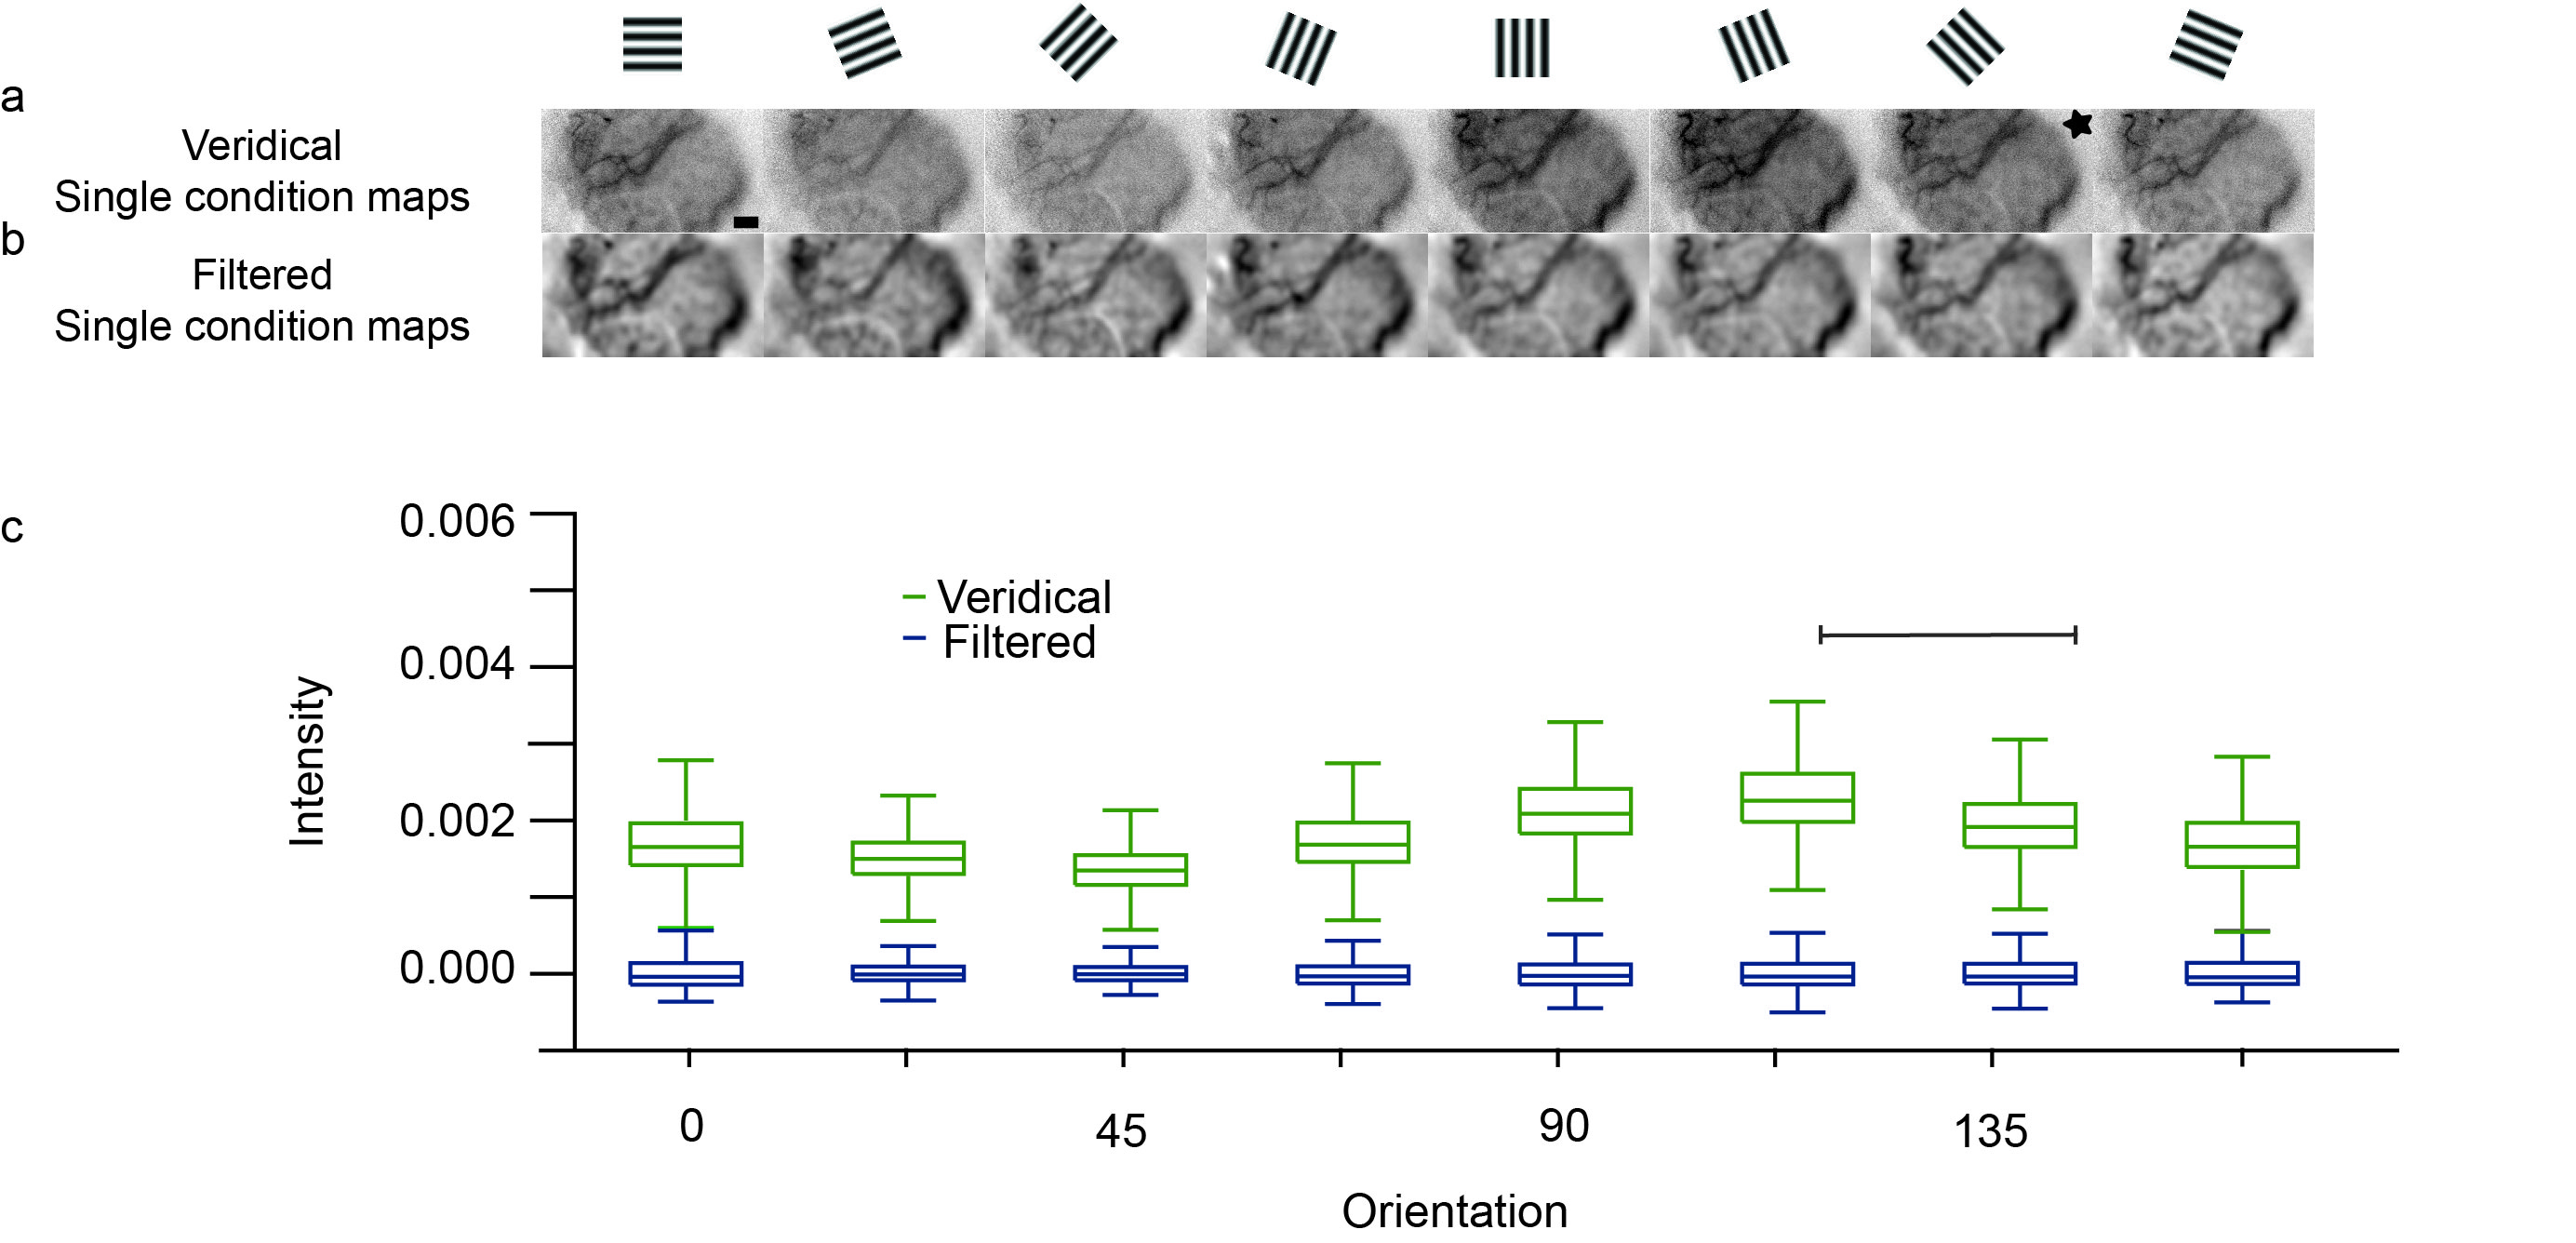
\includegraphics[width=\linewidth]{rb/scms.jpg}
							\caption{Example of filtered and veridical single condition maps.}
							\label{fig:fig3}
						\end{figure}
		\subsubsection{Orientation Tuning Maps}
			The filtered orientation tuning maps resemble the traditional orientation tuning maps whereas the veridical orientation maps are predominantly tuned to one orientation. Figure 6.4 shows the filtered and veridical orientation tuning maps for the same animal showed in figure 6.3. The filtered orientation map shows orientation columns that converge at a pinwheel centre. The response of the neuron indicated by recordings made at the location indicated by the diamond is shown in panel e. The orientation of this neuron corresponds to the orientation of the column from which it was recorded from. The receptive field locations of the recordings are shown in 6.4b. The pseudo colour scale on the outside of the Cartesian scale is the same scale used in parts c and d. We can see that if we draw a line starting from the centre of gaze, passing through the centre of the receptive field to the colour scale, the colours will correspond to the same colours seen in the veridical map indicating that large areas of the cortex in the veridical maps are tuned to the radial orientation. Results are presented in a similar fashion for all the animals in our study in figure 6.5.
			
							\begin{figure}
								
								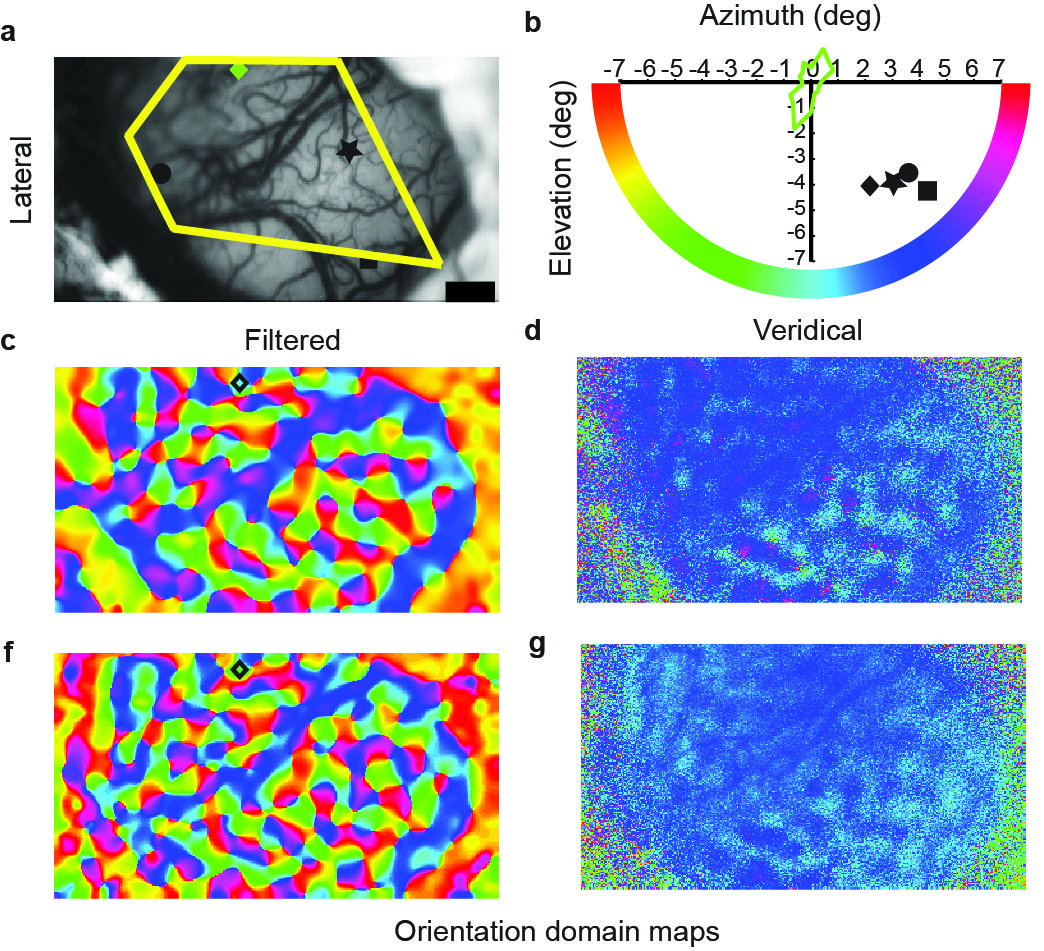
\includegraphics[width=\linewidth]{rb/rep_image.jpg}
								\caption{Orientation maps from a representative animal. (a) is the green image obtained using the 545 nm green filter to show surface landmarks. The yellow polygon is the area used for ROI and single pixel analysis. The various symbols represent the locations of electrode penetrations. The receptive field locations of the electrode penetrations are represented by their corresponding symbol in (b). The orientation tuning curve overlaid on the axis corresponds to the orientation tuning recorded using a tungsten microelectrode from the location denoted by the diamond (coloured green; maximum response= 40 spks/s). The colour of the orientation tuning curve corresponds to the colour of the optimum orientation of the neuron (circular mean= 257 deg) according to the pseudocolor scale. (c) and (d) are the filtered and veridical orientation tuning maps. (e) and (f) are the same maps obtained when the entire experimental protocol is repeated. The diamond’s location is transposed on to the two filtered maps. The optimum orientation obtained from the OI maps was similar to that obtained using electrophysiology (circular mean for OI= 263 deg, average from the two repeats). The optimum orientations of the filtered conditions on the other hand closely correspond to the radial angle of their receptive fields. Scale bar is 1mm.}
								\label{fig:fig4}
							\end{figure}
			
			
			\begin{figure}
				
				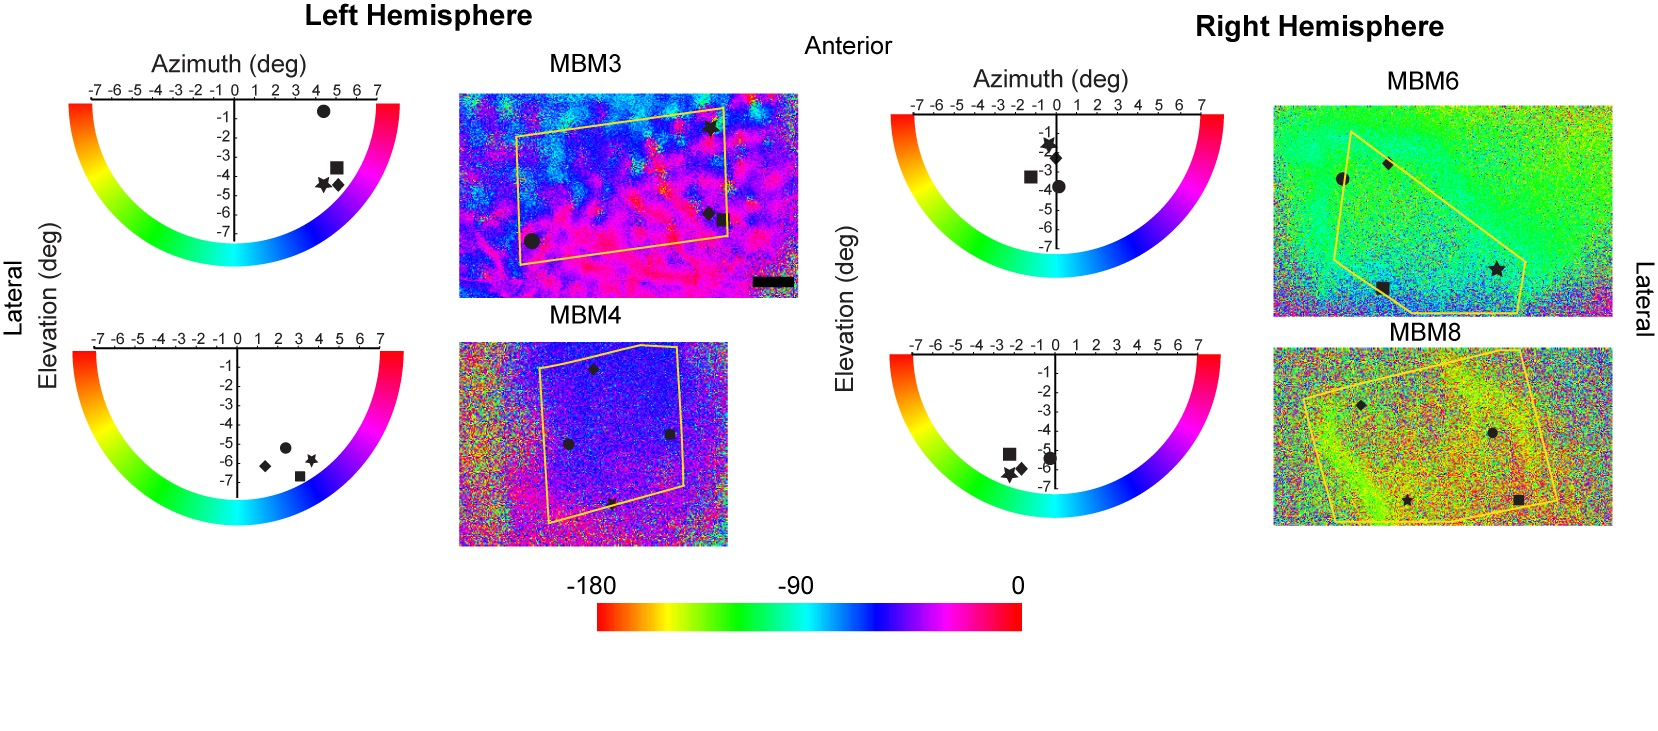
\includegraphics[width=\linewidth]{rb/figure2.jpg}
				\caption{The receptive field location, veridical and filtered orientation tuning maps of  all the animals (except that showed in figure 6.3) used in our studies. The conventions are as explained figure 6.3.}
				\label{fig:fig5}
			\end{figure}
							
		\subsubsection{Comparing the radial orientation and optimum orientation of ROIs}
			When the optimum orientation and the radial orientation were compared, most ROIs were tuned to the radial orientation in the veridical condition. This was not the case in the filtered condition. Figure 6 shows the distribution of the absolute differences between the optimum and radial orientations of the ROIs for the veridical and filtered orientation maps. We find that in the veridical condition, most differences were between 0 and 22.5 degrees (mean=; SE=) suggesting that most of the ROIs were tuned to the radial orientation. In the filtered condition, the mean of the ROIs were further away from zero (mean=; SE=). When a chi-square test was performed, we found that the distribution of absolute differences  for the veridical condition was significantly different from a uniform distribution (chi-square=; df=; p). Surprisingly, the absolute differences for the filtered condition were also significantly different from the uniform distribution but to a lesser extent than the veridical condition (chi-square=; df=;p=). The absolute differences for the veridical and the filtered conditions were also significantly different from each other.
			
			
			\begin{figure}
				
				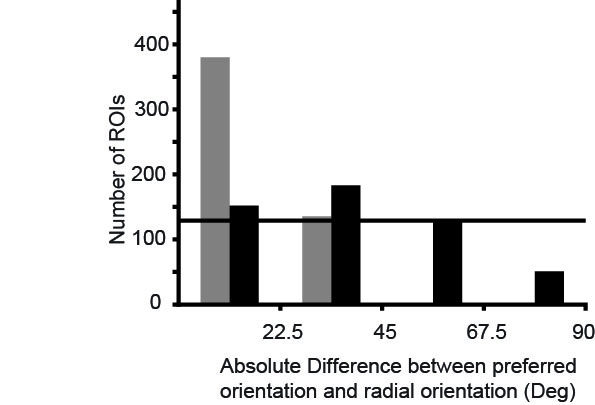
\includegraphics[width=\linewidth]{rb/roi_hist.jpg}
				\caption{The distribution of absolute differences between the optimum orientation of the ROIs and their corresponding radial orientations. The horizontal line indicates the number of ROIs that would be present in each bin if the distribution were uniform.}
				\label{fig:fig6}
			\end{figure}
		\subsubsection{Comparing the radial orientation and optimum orientation of single pixels}
			The difference between the optimum orientation of individual pixels and the mean radial orientation of the imaged area also showed that most pixels in the veridical condition were tuned to the radial orientation. Figure 7 shows the distribution of differences between the individual pixels and the mean radial orientation for the veridical and the filtered conditions. Once again, there was a strong peak between 0 and 22.5 degrees in the veridical condition. There was also a strong response between 22.5 and 45 degrees away from the radial angle. When compared with a uniform distribution (indicated by the horizontal line); the distribution of the differences for the veridical condition was significantly different (chi-square=; df=; p).
			
			
			The difference between the optimum orientation of individual pixels and the mean radial orientation of the imaged area in the filtered condition interestingly showed two peaks; one at the radial orientation and one at the orientation orthogonal to the radial orientation (see figure 7). This distribution was significantly different from the uniform distribution and also the distribution of differences for the veridical condition. When the distributions from the individual animals were fit  with a circular Gaussian distribution, we observe two broadly tuned peaks at 0 degrees and 90 degrees, further emphasising the effect observed in the histograms.
			
			We did not find any significant biases for horizontal and vertical orientations in either the ROI or the single pixel data.
			
				\begin{figure}
					
					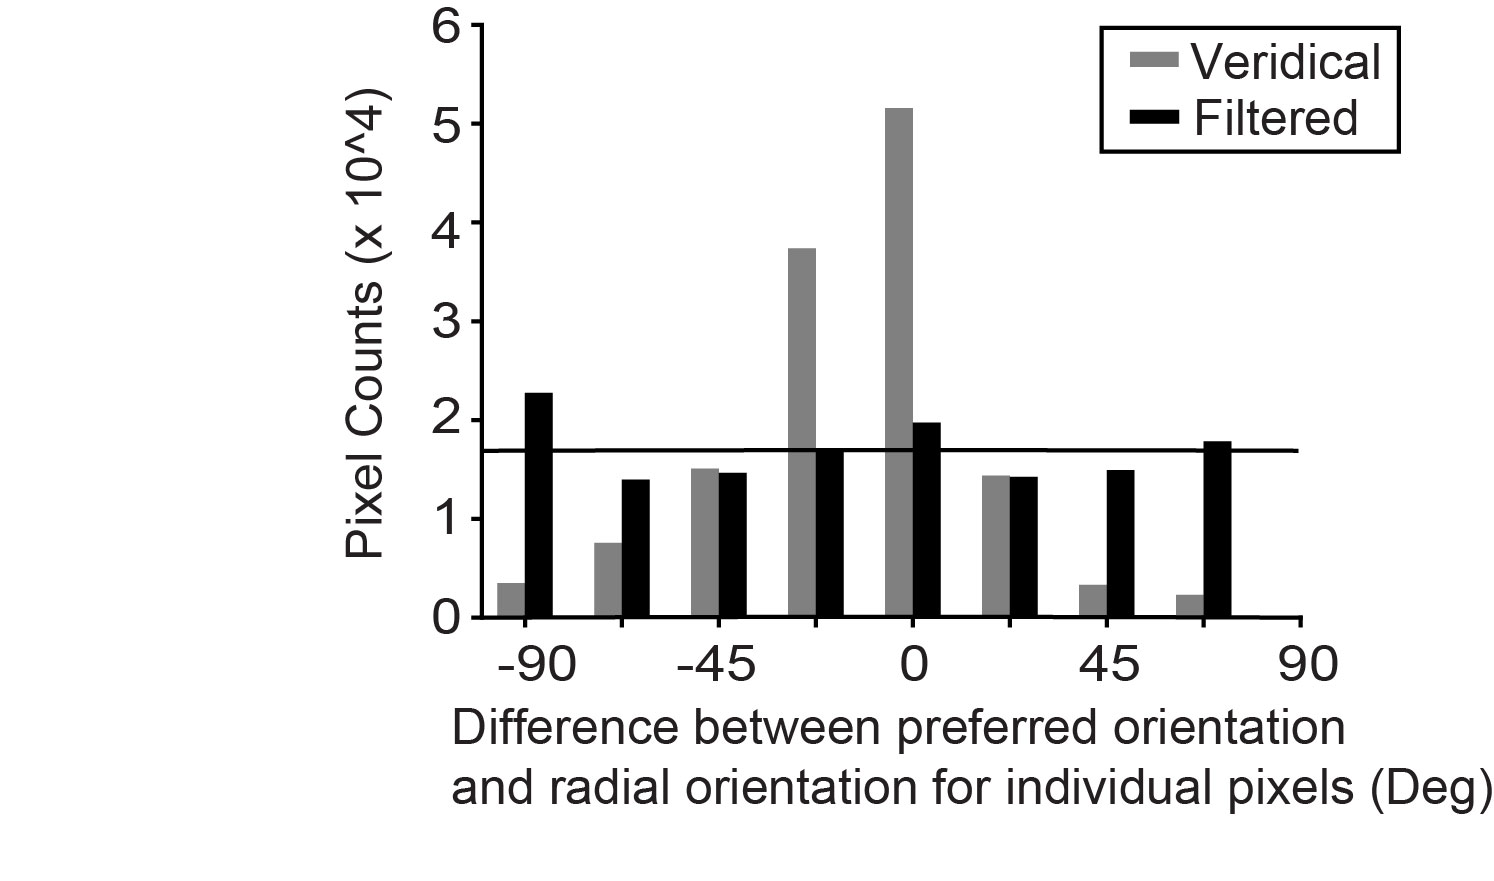
\includegraphics[width=\linewidth]{rb/singlepx_hist.jpg}
					\caption{(a) The distribution of differences between the optimum orientation of single pixels and the mean radial orientation of the imaged area for the veridical and the filtered conditions. (b) The distribution of optimum orientation of the individual pixels grouped according to their preferred orientation. While there is a radial bias in the distribution of the pixels, there is no horizontal or vertical orientation biases.}
					\label{fig:fig7}
				\end{figure}
			
			One important issue that needs to be addressed is the sample size. Figure 7a shows that when looking at single pixels, the sample size is large (on the order of 10\^5 pixels). The chi-square test, when performed on such a large sample will always give a significant result (REFERENCE). Therefore, to make sure that our single pixel results were not an artefact of sample size, we used random, repeated sampling with replacement methods. We used two sample sizes (either 40 or 1000) and sampled 1000 times (1000 trials). The results indicate that the radial bias observed in the veridical maps were strong and were observed even in the condition with sample size=40 (mean chi-square=; p=). There was also significant bias observed with sample size= 1000. For the filtered condition, the biases for the radial and the orthogonal orientation were only visible when sample size was set at 1000. These results indicate that the radial bias in the veridical orientation maps was stronger than the biases observed in the filtered condition. 
				
				\begin{figure}
					
					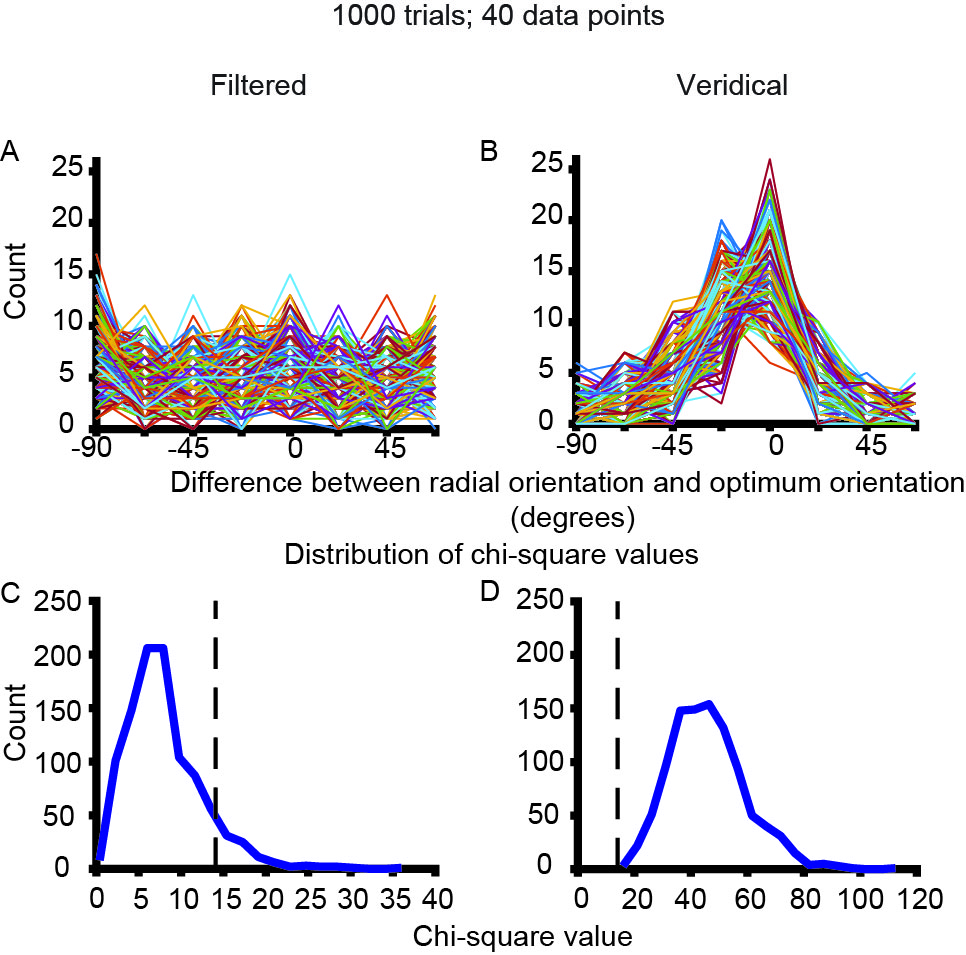
\includegraphics[width=\linewidth]{rb/S3.jpg}
					\caption{Repeated sampling with replacement. Sample size= 40. Number of trials= 1000. (a) and (b) are the distribution of single pixels randomly sampled from the distribution in figure 7a for the filtered and the veridical maps. Each line is the response of the pixel to a particular orientation. Parts (c) and (d) show the distribution of chi-square values for the individual neurons. The vertical line is the chi-square critical value for the given sample size and the degrees of freedom. For the filtered condition, most pixels were uniformly distributed. For the veridical condition, most pixels were significantly different from a uniform distribution.}
					\label{fig:fig8}
				\end{figure}
				
				\begin{figure}
					
					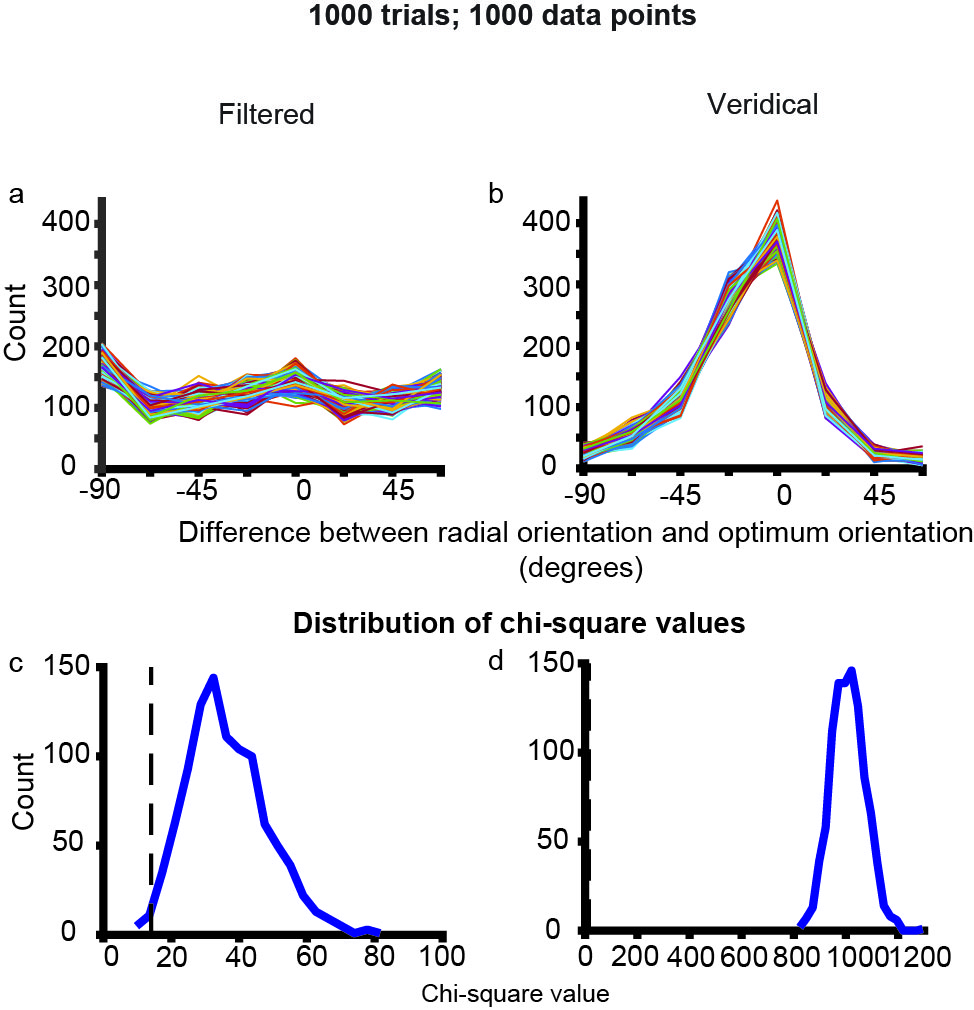
\includegraphics[width=\linewidth]{rb/S4.jpg}
					\caption{Repeated sampling with replacement. Sample size=1000. Number of trials= 1000. (a), (b), (c) and (d) are the same as in Figure 8. When the sample size is increased to a 1000 samples, both the filtered and veridical distributions were significantly different from a uniform distribution.}
					\label{fig:fig9}
				\end{figure}
				
	
				\pagebreak
				
	\section{Discussion}
		
		Using optical imaging of intrinsic signals, we examined the inputs to the primary visual cortex and found that inputs to the primary visual cortex were strongly biased for the radial orientation. This fits in with the hypothesis that the orientation bias observed in the inputs were derived from biases observed in the retina rather than being generated by excitatory convergence of unoriented LGN inputs arranged in a row. However, we predicted that we would observe a bias for more than one of the cardinal orientations. This was not evident in the veridical signal. The filtered signal however, showed a bias to the radial orientation and the orientation orthogonal to the radial orientation. Not sure what this is about.
		
		
		The mean difference between the radial angle and the optimum orientations in both the single pixel and ROI data is significantly different to 0. This indicates that the bias may not be entirely radial. However, this may not necessarily be the case. The experiment could have introduced systematic errors in various stages of data collection and analysis. The plotting of the foveal location is dependent on the visibility of the fovea when observed through the fundus camera. The visibility of the fovea itself is dependent on the optics which tends to deteriorate as the experiment progresses. The determination of the optic nerve head location is more robust. So, as long as an initial estimation of the optic nerve and the fovea are accurate, the subsequent positions of the fovea may be fairly accurately determined by plotting the ON.
		
		
		Receptive field estimation is also subject to error. Dow et al., allow for a half a degree jitter in both receptive field position and size of the receptive field. This compared with the fact that the ROI centres are extrapolated from the RF measurements could introduce another element of error. The formula used for extrapolation itself may not be exactly accurate in every animal and only allow for a crude extrapolation of receptive field position. This is because there are large variances in the organisation of the cortex between macaques and the estimates of RF location are based on standardised values. These differences may also introduce a systematic error in individual animals which could also add up.
		
		Further, the single pixel optimum orientations were all compared to the mean radial angle of the imaged area. The radial angles of the receptive fields in the imaged area on area vary up to 30 degrees depending on the eccentricity of imaging. This introduces a further element of error in the measurements which contribute to a larger spread of differences in the single pixel data. Taking into account all these sources of error in determining the difference between the radial angle and optimum orientation, the actual radial bias in the data may be stronger than what has been reported.
		
		
		During imaging, the tandem lens arrangement allows us to focus on a very narrow plane under the surface of the cortex while imaging. This depth is usually chosen on the basis of a few different factors. First, we need to see at what depth the signal we are looking for is strongest. The inputs to the macaque cortex arrive in layer 4. Layer 4 is approximately 900 microns below the surface of the cortex. Imaging at these depths requires long wavelength filters. However, at these longer wavelengths, there is an increase in noise due to light scattering. The longest wavelengths that have been used for optical imaging are in the infrared range (~710 nm) and at these wavelengths, the largest component of the signal is the noise caused by light scatter. Therefore, a trade-off needs to be made between depth and wavelength of the filter. In this study, we used a 630 nm filter and focussed our camera at a depth of 550-700 microns. This lets us image the bottom of layer 2/3. Layer 2/3 receives inputs from layer 4 but studies have shown that no further sharpening of orientation occurs in the parvocellular layer of layer 4 and there are also direct, koniocellular inputs to layer 2/3 in the macaque V1. Therefore, we can measure the pre-synaptic and synaptic inputs to layer 2/3 and still reliably make inferences on the nature of the inputs to the visual cortex itself.
		
		
		Other optical imaging studies that have examined orientation biases have demonstrated the oblique effect; that is an underrepresentation of the oblique orientations in the primary visual cortex.  These studies examined biases by grouping pixels based on their responses to different orientation but did not examine their relationship with their receptive field locations. Where the relationship between the receptive field location and the orientation of the neurons was, a radial bias was reported every time and at every stage of the visual system. In some cases, a horizontal bias has been reported due to the presence of the horizontal streak in the retina but even in these animals, as one goes further away from the horizontal streak and the fovea, a strong radial bias is observed.
		
		
		The radial bias might be an inevitable effect in the visual system. The prevalence of the radial bias has been higher in the peripheral visual system. Psychophysical studies have shown that the oblique effect is a very strong effect. The neurophysiological correlates of these oblique effects have been unclear but the radial bias in the periphery seems to be a result of the way in which the eye grows, automatically elongating the ganglion cell dendritic fields which influence their responses to oriented stimuli. The oblique effect in perception and the radial bias on the neural level may be unrelated phenomena.
	
	
		Recent fMRI studies have demonstrated the radial bias in the visual cortex. Studies by Sasaki et al, etc have shown that when shown obliquely oriented stimulus, the activity in the BOLD response is higher than that observed for the horizontal and vertical stimuli. These studies show the radial bias on a larger and cruder spatial scale. Here, the radial bias in the cortex has been demonstrated at a smaller scale and a higher resolution, relating optimum orientations to receptive field locations rather than whole hemispheres. Sasaki et al. (2006) also demonstrate that the radial bias exists at higher visual areas. Our own results suggest that the inputs to the extrastriate areas from V1 will be tuned to the radial and the orthogonal orientations. These results along with our results indicate that the radial bias plays an important role in establishing cortical architecture.
		
		If the range of orientation selectivity seen in the primary visual cortex originates from biases observed in the subcortical areas, we predicted that the inputs to the cortex may be broadly tuned to a small number of orientations. According to our results, one orientation dominated the inputs to the cortex. This does not necessarily mean that only one orientation is present in the inputs. The magnitude of the radial orientation signal is large and might overwhelm any smaller biases that may be observed. There would be no way to separate these signals on a spatial scale (as we usually do with the extracellular signal) without losing the information. A temporal means of segregating these signals may exist but again, our temporal resolution is not high enough to observe these changes. Our results only show that the inputs to the V1 are dominated by the radial orientation.
		 
	\pagebreak
	\section{Conclusions}
	
		In this chapter, we aimed to examine if the inputs to the macaque primary visual cortex were predominantly tuned to a cardinal orientation. We used the unfiltered signal obtained from optical imaging of intrinsic signals in order to examine the larger scale organisation of the inputs. We imaged lower layer 2/3 and found that the presynaptic and synaptic activity were predominantly tuned to the radial orientation. The filtered signal was tuned to the radial and the orientation orthogonal to the radial orientation. Our results indicate that the columnar organisation observed in the primary visual cortex can be derived from biases observed in the subcortical areas and that excitatory convergence is not the source of orientation biases observed in the cortex.
		